\documentclass[10pt]{article}

% %%%%%%%%%%%%%%%%%%%%%%%%%%%%%%%%%%%%%%%%%%%%%%%%%%%%%%%%%%%%%%%%%%%%%%%%%%%%%%
% %                                 PACKAGES                                   %
% %%%%%%%%%%%%%%%%%%%%%%%%%%%%%%%%%%%%%%%%%%%%%%%%%%%%%%%%%%%%%%%%%%%%%%%%%%%%%%
% Identifies input coming with an UTF-8 format
\usepackage[utf8]{inputenc}
% Uses 8-bit T1 fonts (Latin) 
\usepackage{setspace}
 \singlespacing
% Arial font.
\usepackage[scaled]{helvet}
\renewcommand\familydefault{\sfdefault}
\usepackage[T1]{fontenc}
\setlength{\parindent}{0.4cm}
% Equations
\usepackage{amsmath}
% Enum Item
\usepackage{enumitem}
% Easy Lists
\usepackage[ampersand]{easylist}
% Tables
\usepackage{booktabs}
\usepackage{longtable}
% Hyperreferences
\usepackage{hyperref}
% Images
\usepackage{graphicx}
% Set images location
\usepackage{wrapfig}
% Position for tables and images
\usepackage{float}
% Blibliography
\usepackage[backend=biber, style=numeric]{biblatex}
 \addbibresource{paper.bib}

\begin{document}

\title{PL3 - Cloud Computing}

\author{Pablo Acereda \and
David E. Craciunescu \and
Ángel Martín \and
Ángelo Moreno \and
Laura Pérez
}

\institute{Universidad de Alcalá de Henares - EPS}

\maketitle

\section{Contenedores}

\section{IA \& Machine Learning}

\section{IoT}

Partiendo de una definición base, IoT (Internet of Things) es el conjunto de
dispositivos que forman una red, la cual permite el intercambio de información y
datos entre terminales.

Una vez que se tiene una cierta noción de lo que es IoT, es hora de pasar al
desarrollo llevado a cabo en las dos plataformas empleadas: Microsoft Azure y
Amazon Web Service.

Como última adenda a esta cuestión, decir que van a incluirse capturas de los
procesos llevados a cabo, y para demostrar la realización del trabajo.

\subsection*{Microsoft Azure}

A continuación, van a ser descritos los pasos realizados para controlar un
dispositivo conectado a IoT Hub, uno de los servicios encontrados en Microsoft
Azure.

\subsubsection{Prerrequisitos}

Como puede ser comprensible, no todo es tan sencillo como ponerse a escribir y
conseguir un resultado de manera directa, primero es necesario que el
dispositivo que va a emplearse está preparado con las aplicaciones y
herramientas necesarias.

Para ello, hay que asegurarse de que haya instalado una versión de Node.js en el
dispositivo. En caso de no saber si se cuenta con una instalación de Node.js, es
 tan sencillo como ejecutar el siguiente comando
 \hyperref[eq:command]{\ref{eq:command}}:

\begin{equation}
 \label{eq:command}
node --version
\end{equation}

Si se cuenta con una versión (acorde a la documentación oficial
\cite{azure_iot}) igual o posterior a 4.x.x será necesario descargarla de la
que puede encontrarse en \cite{node} 
\hyperref[downloadnode]{\ref{downloadnode}}. Cabe añadir que Node.js no es la 
única tecnología que puede emplearse para este desarrollo, debido a que también
se acepta: .NET, Java, Python y Android; pero por elección del desarrollador de
este apartado se ha decidido emplear Node.js.

\begin{figure}[h!]
 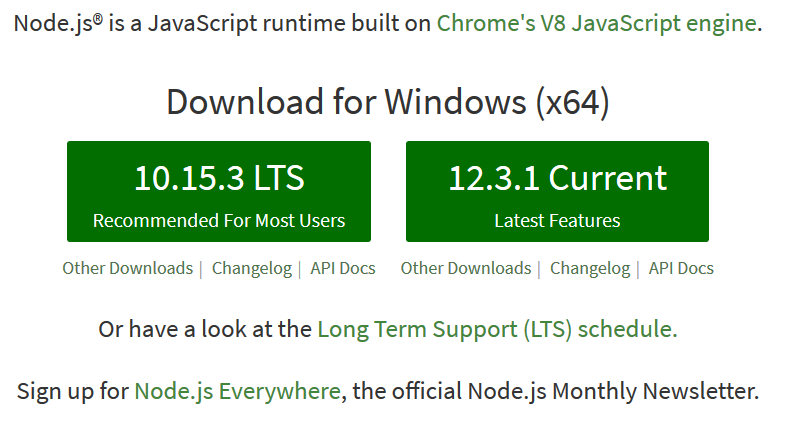
\includegraphics[width=\linewidth]{./IoT/MicrosoftAzure/4-3-1_send_simulated_telemetry.png}
 \caption{Descarga de Node.js desde el sitio web oficial.}
 \label{downloadnode}

\end{figure}

Acorde a la documentación, también es necesario ejecutar el comando
\hyperref[eq:azurecli]{\ref{azurecli}}

\begin{equation}
 \label{eq:azurecli}
 az extension add --name azure-cli-iot-ext
\end{equation}

El cual agrega la extensión IoT de Azure para la CLI a la instancia de Cloud
Shell.

Por último, en caso de no contar con un dispositivo que conectar, siempre puede
emplearse lo proporcionado en 
\url{https://github.com/Azure-Samples/azure-iot-samples-node/archive/master.zip}

\subsubsection{Creación de un centro de IoT}

Dentro de Azure portal, cuyo acceso no merece mención debido a la experiencia
por parte del lector en este tema, se busca ``IoT Hub'' en la barra situada en
la parte superior del portal.

Una vez dentro de IoT Hub, se crea un nuevo recurso. La pantalla debería quedar
tal y como se puede ver en la captura
\hyperref[createresource]{\ref{createresource}}. Es necesario seleccionar el
grupo al cual pertenecerá el nuevo recurso y, en caso neceasrio, crear uno
nuevo. Por último, se selecciona un nombre para el IoT Hub (en este caso se ha
decidido que sea Hefesto, por ser el dios griego del fuego, la forja y los
artesanos; al ser el desarrollador que replique este proceso el que de forma y
esculpa el funcionamiento del dispositivo).

\begin{figure}[h!]
 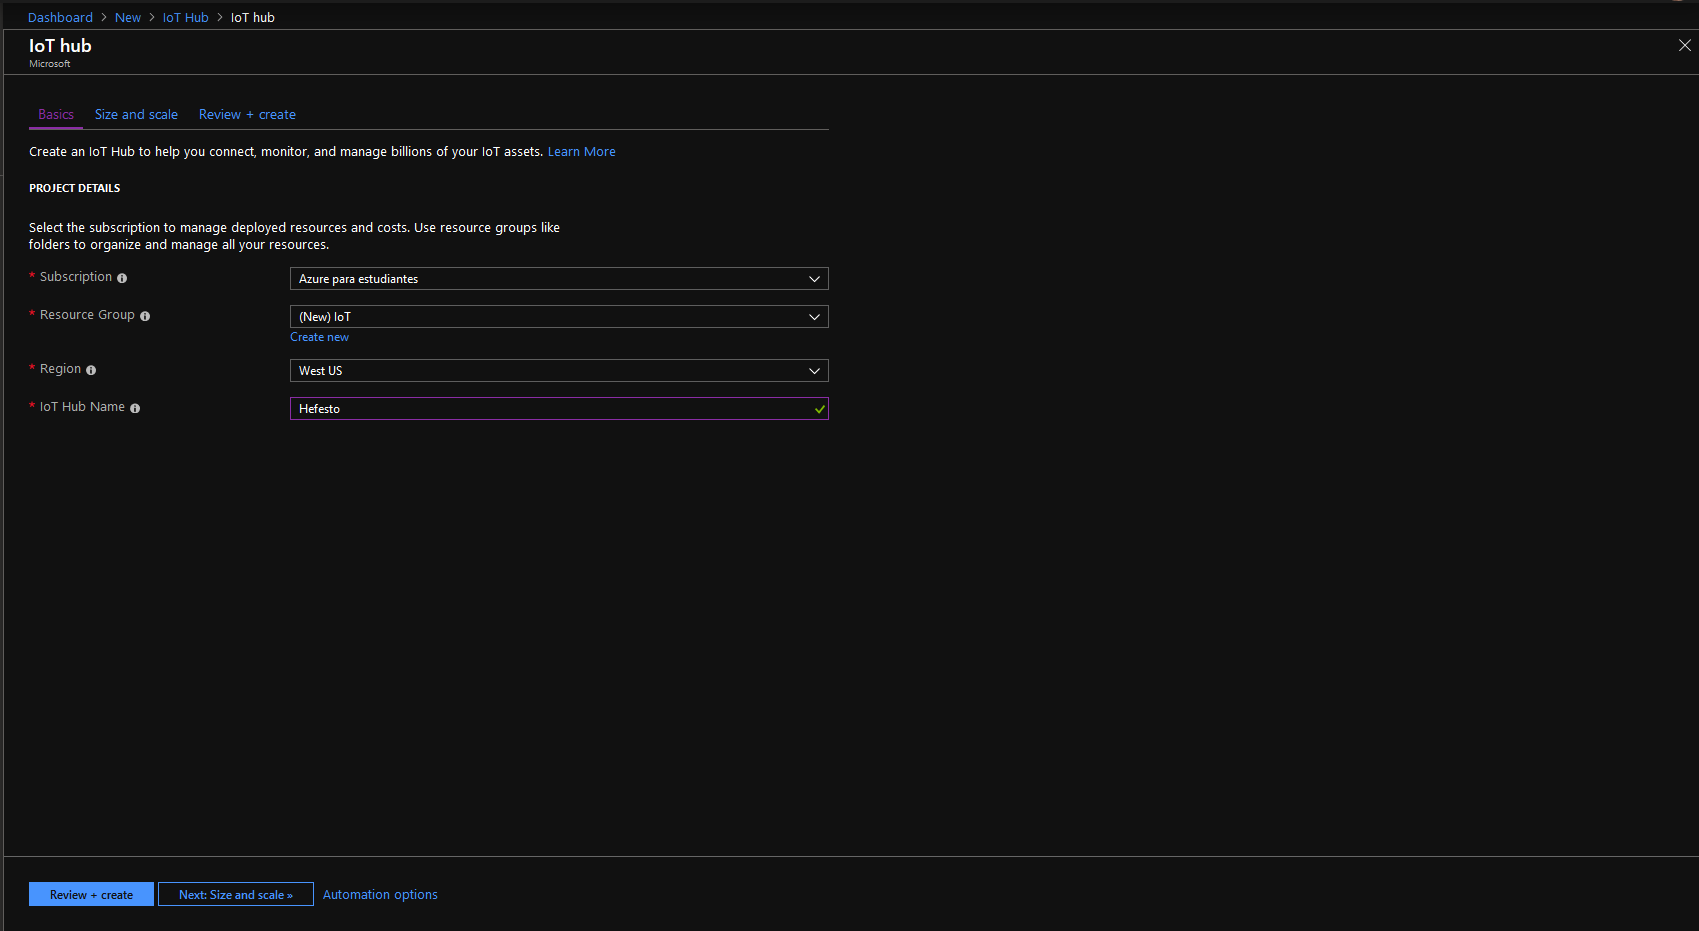
\includegraphics[width=\linewidth]{./IoT/MicrosoftAzure/1-1_create_resource.png}
 \caption{Inicio del proceso de creación de recurso: asignación de Grupo y
 Nombre.}
 \label{createresource}
\end{figure}

Una vez finalizados los pasos de la explicación anterior, se pasa al siguiente
punto, definición del tamaño y la escala \hyperref[sizescale]{\ref{sizescale}}.
En esta página, tal y como su nombre indica, se seleccionarán el tamaño (número
de unidades) y la escala (de entre las que proporciona Microsoft Azure). De las
escala, cabe añadir que se encuentran los siguientes tipos:

\begin{easylist}[itemize]
  & Estándar (desde S1 hasta S3).
  & Básico (desde B1 hasta B3).
  & Gratuito. De este cabe decir que solo se emplea para pruebas y evaluaciones.
  Permite 500 dispositivos con el centro de IoT y hasta 8000 mensajes al día.
  Solo puede crearse una instacia \cite{azure_iot}.
\end{easylist}

\begin{figure}[h!]
 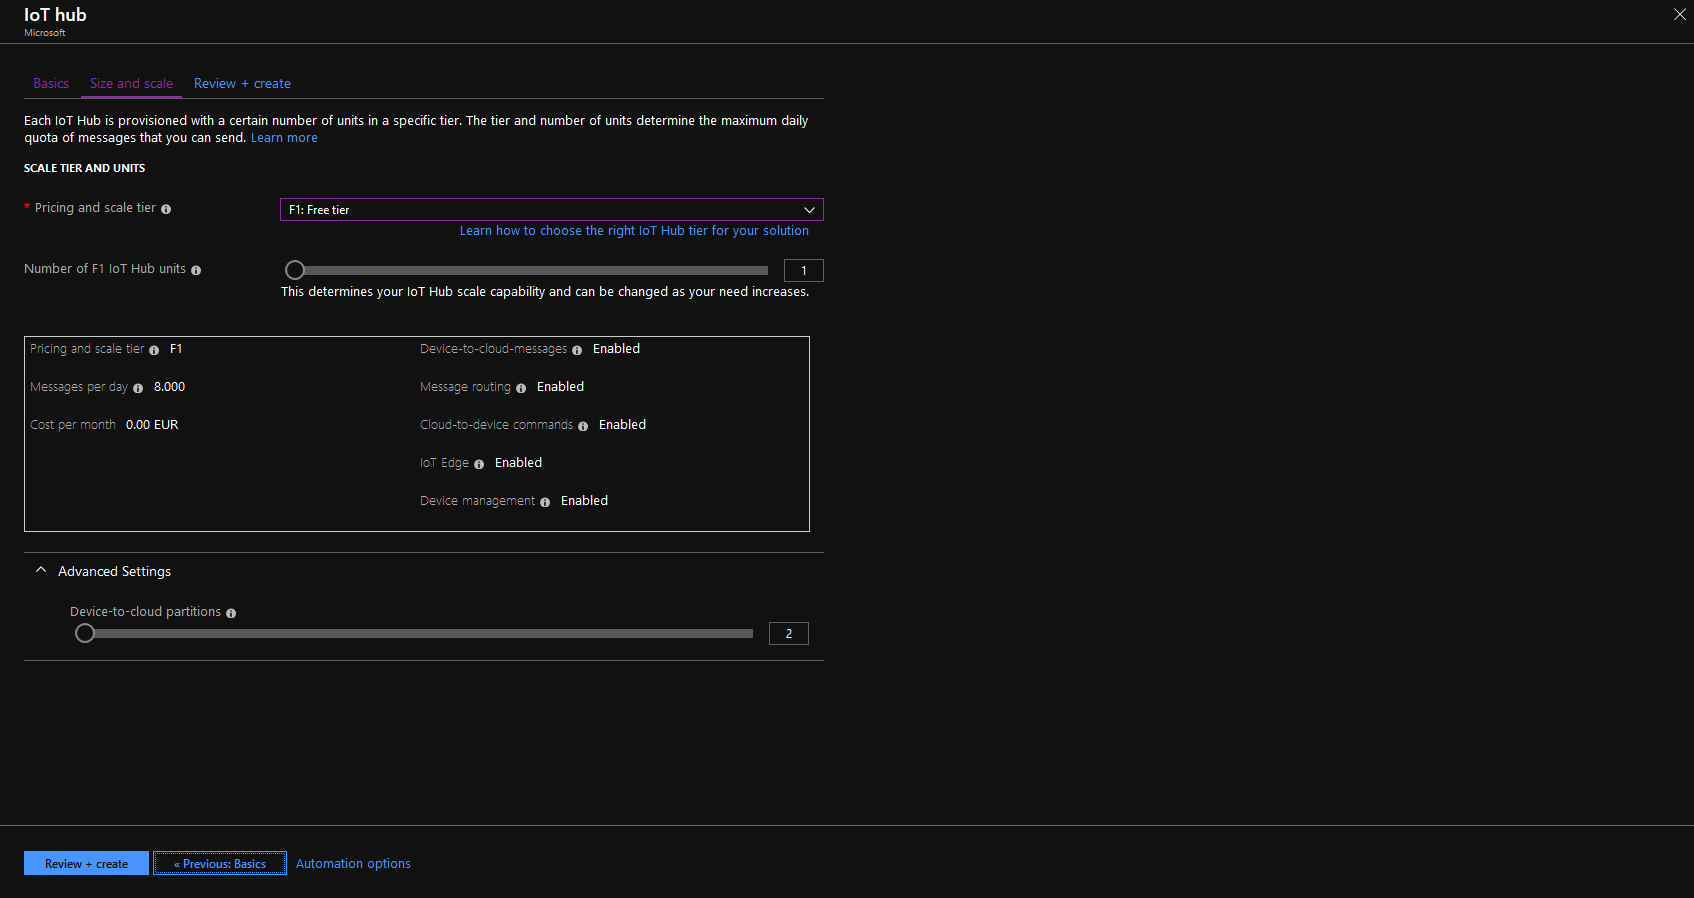
\includegraphics[width=\linewidth]{./IoT/MicrosoftAzure/1-2_create_resource.png}
 \caption{Seleccionar tamaño y escalabilidad}
 \label{sizescale}
\end{figure}

Se puede pasar a revisar y crear la unidad IoT Hub \hyperref[review]{\ref{review}}.

\begin{figure}[h!]
 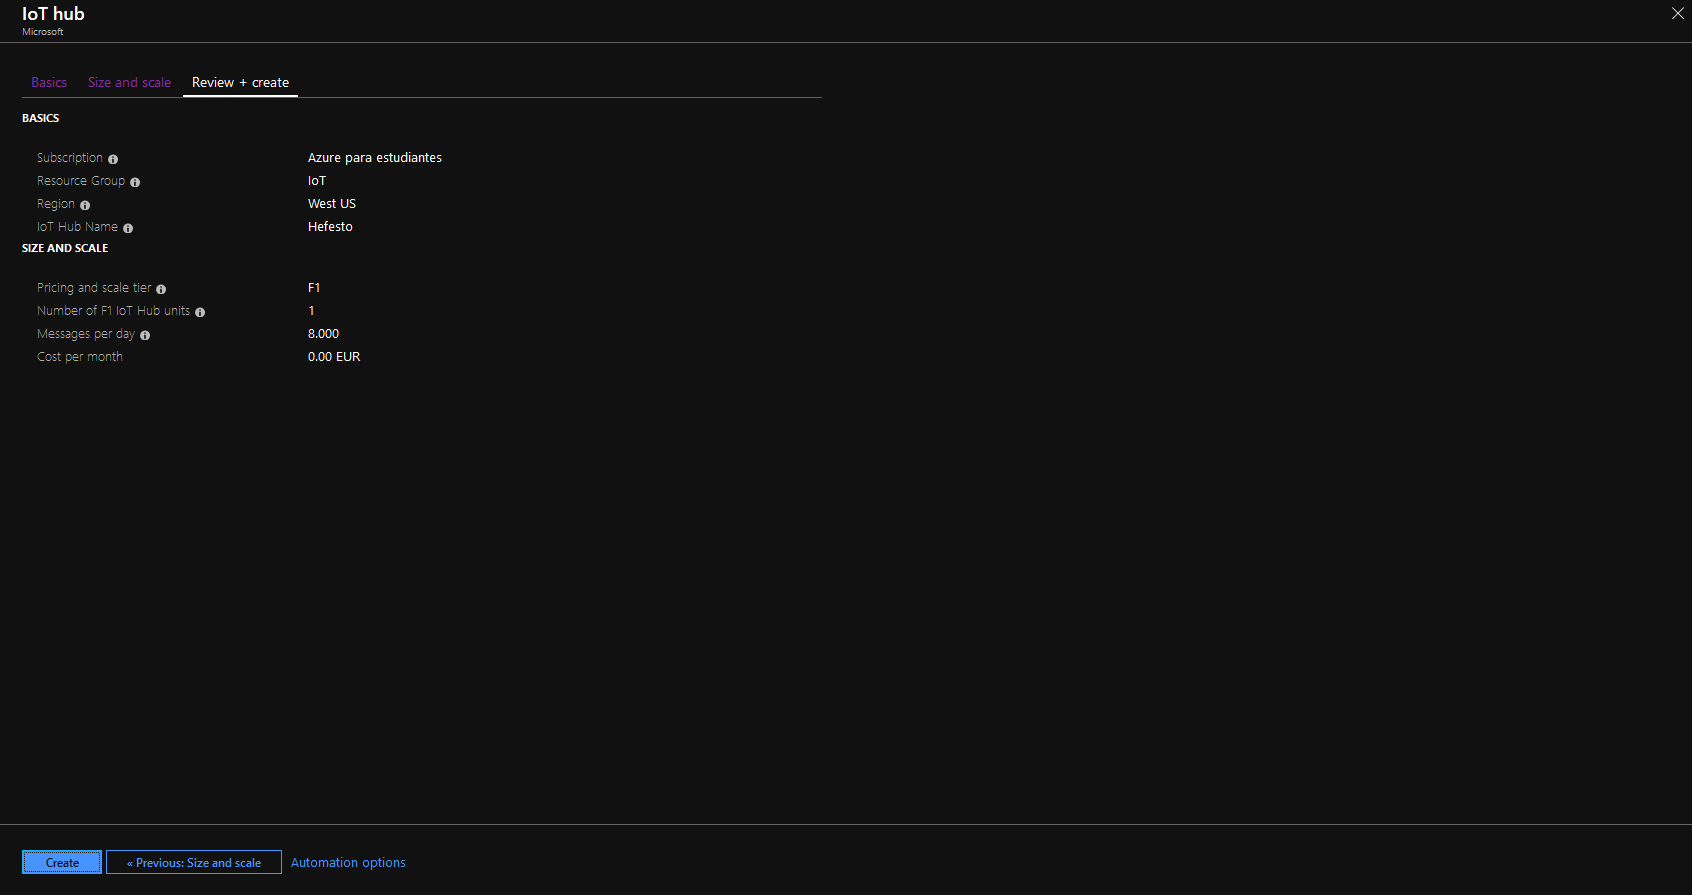
\includegraphics[width=\linewidth]{./IoT/MicrosoftAzure/1-3_create_resource.png}
 \caption{Revisión y Creación.}
 \label{review}
\end{figure}

\subsubsection{Registrar Dispositivo}

Para registrar el dispositivo que se va a emplear, es necesario acceder a la
terminal de Azure. No se va a proporcionar ninguna explicación de como acceder a
la misma, debido a que el lector ya es consciente de como llegar hasta ella.

Primero, se debe empezar por crear la identidad del dispositivo 
\hyperref[register]{\ref{register}}, con la que será referido a partir de ahora 
mediante el comando:

\begin{equation}
 \label{deviceid}
 az iot hub device-identity create --hub-name YourIoTHubName --device-id 
 MyNodeDevice
\end{equation}

Dentro de \hyperref[deviceid]{\ref{deviceid}} se debe sustituir YourIoTHubName
por el nombre del Hub, que en este caso será Hefesto; y MyNodeDevice por el
nombre del dispositivo, se ha dejado tal cual por mera comodidad, al tener esta
práctica como objetivo aprender a usar las nociones básicas de las plataformas
Cloud.

Al ejecutar queda la siguiente traza \hyperref[register]{\ref{register}}:

\begin{figure}[h!]
 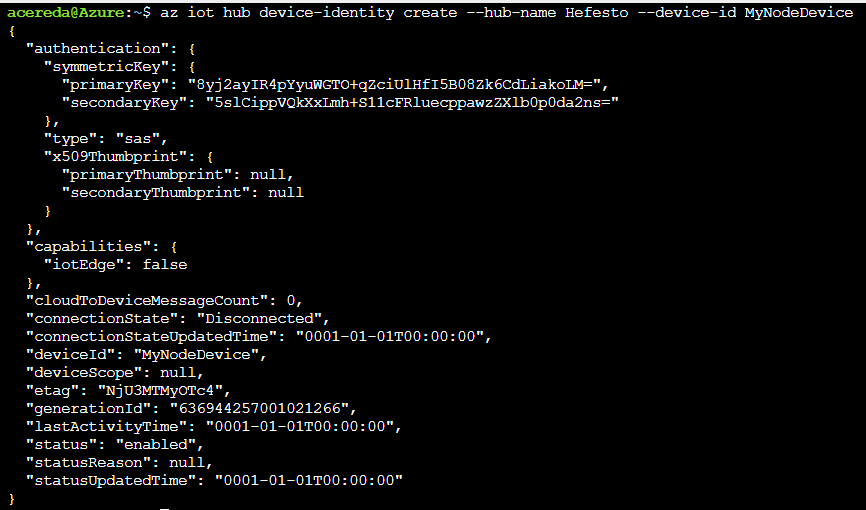
\includegraphics[width=\linewidth]{./IoT/MicrosoftAzure/3-1_register_device.png}
 \caption{Registro del dispositivo.}
 \label{register}
\end{figure}

Acto seguido, se debe conseguir la cadena de conección perteneciente a al
dispositivo. Una vez más, se debe ejecutar en la consola un comando:

\begin{equation}
 \label{condevcommand}
 az iot hub device-identity show-connection-string --hub-name YourIoTHubName 
 --device-id MyNodeDevice --output table
\end{equation}

Una vez más, se sustituye YourIoTHubName por Hefesto, que es al que se quiere
hacer referencia. La cadena resultante de la ejecución del comando debe 
guardarse \hyperref[constring]{\ref{constring}} para, posteriormente, poder 
realizar la conexión con el disposito.

\begin{figure}[h!]
 \includegraphics[width=\linewidth]{./IoT/MicrosoftAzure/3.2_register_device.png}
 \caption{Conexión con el dispositivo.}
 \label{constring}
\end{figure}

Finalmente, se debe hacer de manera similar, pero en este caso con la cadena de
conexiónde servicio. Este último permite conectarse al IoT Hub y recuperar los
mensajes enviados por el dispositivo.

\begin{equation}
 \label{consercommand}
az iot hub show-connection-string --name YourIoTHubName --output table
\end{equation}

\subsubsection{Envío de datos de telemetría simulados}

Todo lo hecho anteriormente está muy bien y tal\ldtos, pero no es una
``aplicación real''. El dispositivo debería poder mandar datos al fin y al cabo.
Para ello se debe abrir una terminal local, e ir al directorio donde se ha
descargado, en este caso, el ejemplo del repositorio Git proporcionado
anteriormente en este documento. Se debe entrar al directorio
\textit{iot-hub\\Quickstarts\\simulated-device}
\hyperref[directory]{\ref{directory}}.

\begin{figure}[h!]
 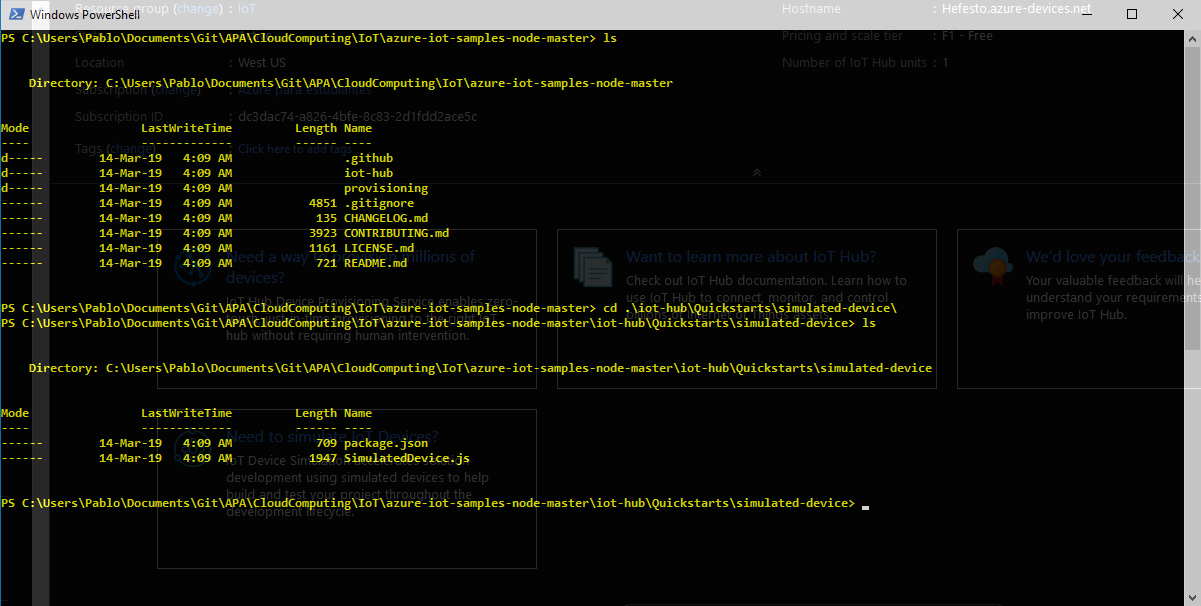
\includegraphics[width=\linewidth]{./IoT/MicrosoftAzure/4-1_send_simulated_telemetry.png}
 \caption{Conexión con el dispositivo.}
 \label{directory}
\end{figure}

Debe sustituirse el contenido de \textit{connectionString}
\hyperref[directory]{\ref{directory}} a la salida obtenida en la ejecución de 
\hyperref[condevcommand]{\ref{condevcommand}} en el archivo SimulatedDevice.js.

\begin{figure}[h!]
 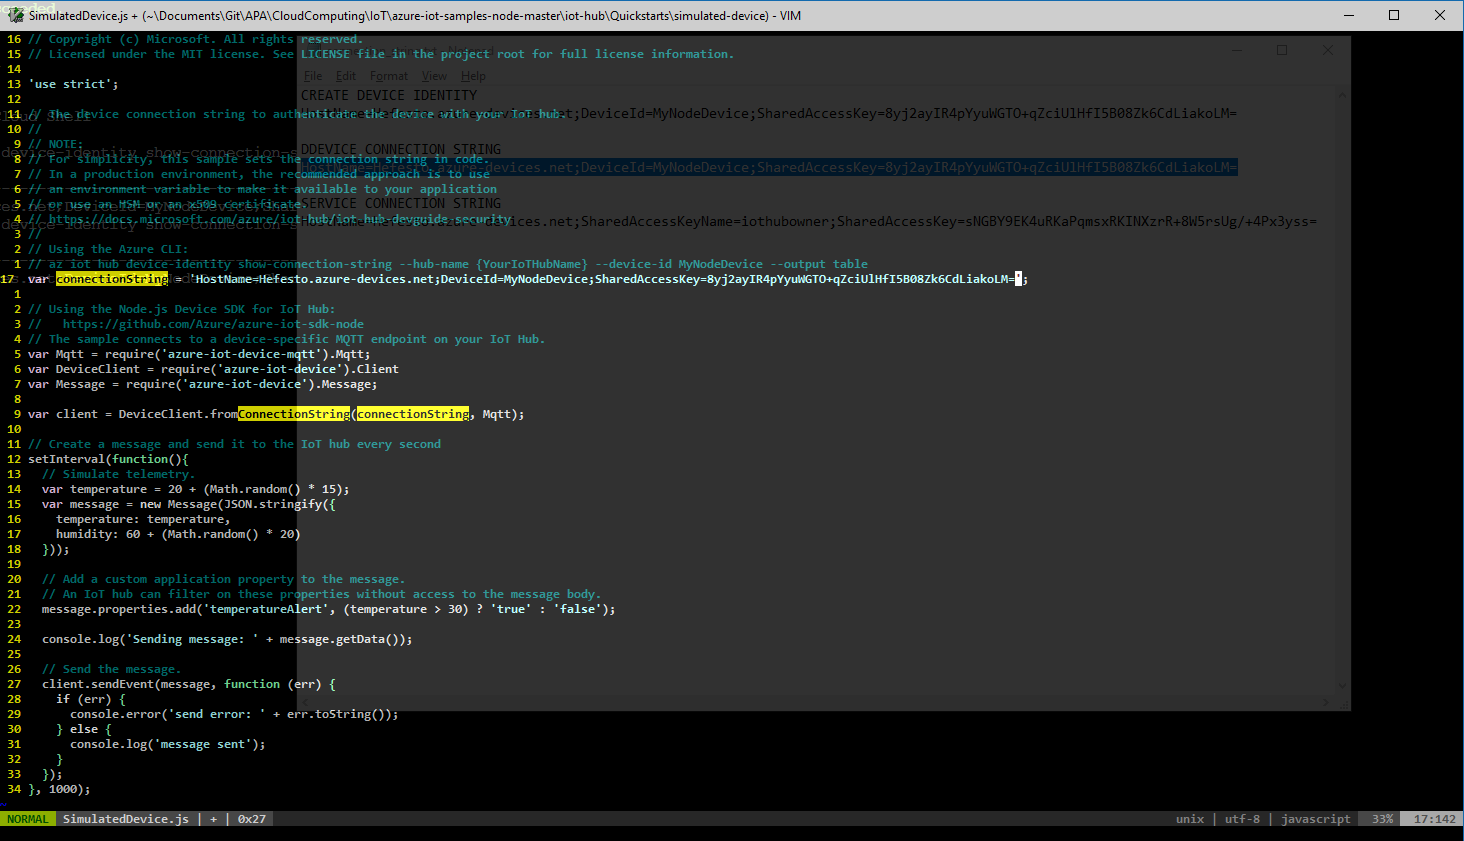
\includegraphics[width=\linewidth]{./IoT/MicrosoftAzure/4-2_send_simulated_telemetry.png}
 \caption{Cadena de conexión del dispositivo.}
 \label{codestring}
\end{figure}

Tras guardar el archivo, ya puede ejecutarse el código:

\begin{equation}
 \label{ejecdev1}
npm install
\end{equation}

\begin{equation}
 \label{ejecdev2}
node SimulatedDevice.js
\end{equation}

\begin{figure}[h!]
 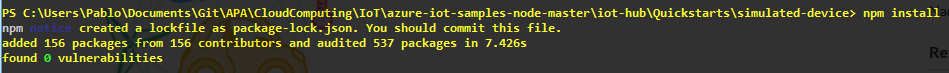
\includegraphics[width=\linewidth]{./IoT/MicrosoftAzure/4-4_send_simulated_telemetry.png}
 \caption{Instalación de paquetes necesarios para la ejecución.}
 \label{npmdev}
\end{figure}

El resultado de la ejecución da el siguiente resultado
\hyperref[nodedev]{\ref{nodedev}}, que como se puede observar hace referencia a 
los mensajes enviados por el disposito.

\begin{figure}[h!]
 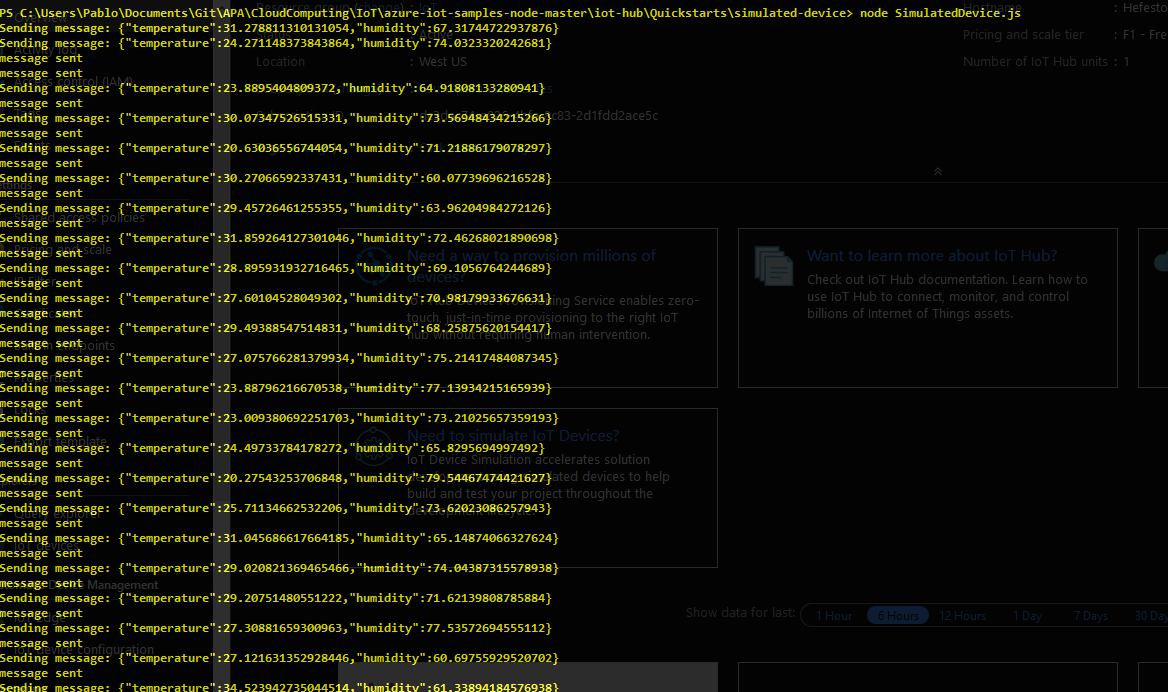
\includegraphics[width=\linewidth]{./IoT/MicrosoftAzure/4-5_send_simulated_telemetry.png}
 \caption{Conexión con el dispositivo.}
 \label{nodedev}
\end{figure}

\subsubsection{Lectura de los datos de telemetríá procedentes de su instancia de
IoT Hub}

Pero no solo hay que mandar datos, también hay que ser capaz de leerlos. En este
apartado se explica como crear un proceso que tome los datos del dispositivo,
desde IoT Hub, y los lea. Para ello hace falta otra instancia de la terminal
local. En este caso, en lugar de la ruta \textit{simulated-device}, se accede a
la ruta \textit{iot-hub\\Quickstart\read-d2c-messages}
\hyperref[directoryreader]{\ref{directoryreader}}.

\begin{figure}[h!]
 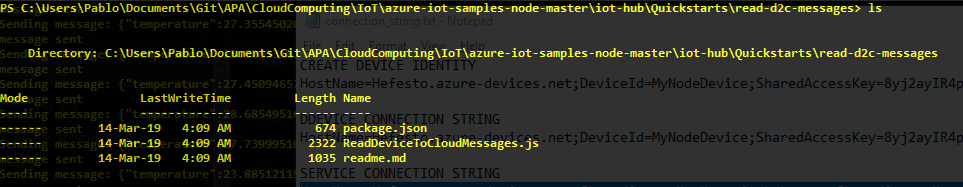
\includegraphics[width=\linewidth]{./IoT/MicrosoftAzure/5-1_read_telemetry.png}
 \caption{Lectura de datos del dispositivo.}
 \label{directoryreader}
\end{figure}

Al igual que en el caso de la escritura de datos, en la lectura de datos es
necesario especificar en el fichero ReadDeviceToCloudMessages.js. En este caso
el contenido de \textit{connectionString} debe sustituirse
\hyperref[codestringser]{\ref{codestringser}} por lo obtenido en la cadena de 
conexión de servicio \hyperref[consercommand]{\ref{consercommand}}.

\begin{figure}[h!]
 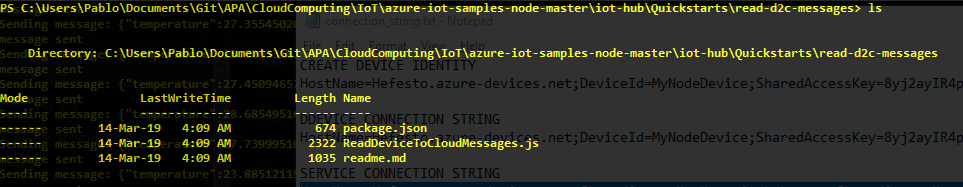
\includegraphics[width=\linewidth]{./IoT/MicrosoftAzure/5-1_read_telemetry.png}
 \caption{Cadena de conexión a servicio.}
 \label{codestringser}
\end{figure}

Una vez más, debe ejecutarse \hyperref[ejecdev1]{\ref{ejecdev1}}, seguido de
\hyperref[ejecdev3]{\ref{ejecdev3}}.

\begin{equation}
 \label{ejecdev3}
node ReadDeviceToCloudMessages.js
\end{equation}

El resultado de la ejecución del comando anterior
(\hyperref[ejecdev3]{\ref{ejecdev3}}) puede observarse en la captura 

\begin{figure}[h!]
 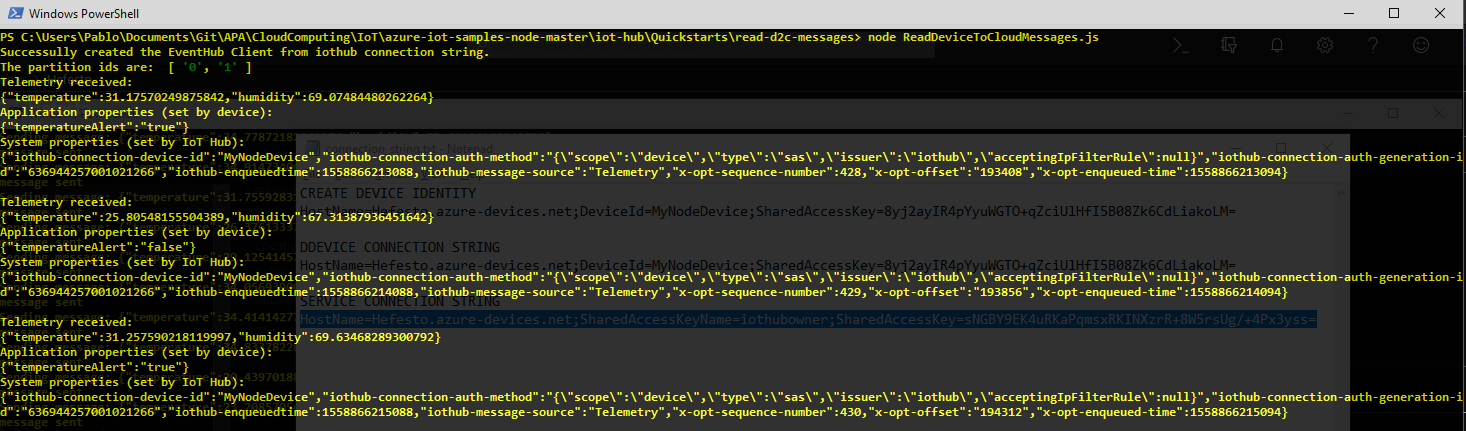
\includegraphics[width=\linewidth]{./IoT/MicrosoftAzure/5-4_read_telemetry.png}
 \caption{Cadena de conexión a servicio.}
 \label{nodeser}
\end{figure}

\subsection*{Amazon Web Service}

\section{Seguridad}

\section{Web \& Logic Apps}

\end{document}

